\documentclass[tikz]{standalone}

\pgfkeys{
  mygrid/.is family,
  mygrid,
  min x/.initial=-5,
  max x/.initial=5,
  min y/.initial=-5,
  max y/.initial=5,
  small step/.initial=.1,
  step/.initial=1,
  big step/.initial=5,
  color/.initial=red,
}
\newcommand\mygridset[1]{\pgfkeys{mygrid,#1}}
\newcommand\mygrid[1][]{
  \mygridset{#1,
    min x/.get=\gridminx,
    max x/.get=\gridmaxx,
    min y/.get=\gridminy,
    max y/.get=\gridmaxy,
    small step/.get=\gridsmallstep,
    step/.get=\gridstep,
    big step/.get=\gridbigstep,
    color/.get=\gridcolor
  }

  \draw [step=\gridsmallstep, help lines,\gridcolor!20]
  (\gridminx,\gridminy) grid (\gridmaxx,\gridmaxy);
  \draw [step=\gridstep, help lines,\gridcolor!40]
  (\gridminx,\gridminy) grid (\gridmaxx,\gridmaxy);
  \draw [step=\gridbigstep, help lines,\gridcolor!100]
  (\gridminx,\gridminy) grid (\gridmaxx,\gridmaxy);
  \foreach \x in {\gridminx,...,\gridmaxx} {
    \node[below,font=\tiny] at (\x,\gridminy) {$\x$};
    \node[above,font=\tiny] at (\x,\gridmaxy) {$\x$};
  };
  \foreach \y in {\gridminy,...,\gridmaxy} {
    \node[left,font=\tiny] at (\gridminx,\y) {$\y$};
    \node[right,font=\tiny] at (\gridmaxx,\y) {$\y$};
  };
}

% a style to memorize some change to the default values
\mygridset{
  a grid/.style={
    min x=-3,
    max x=3,
    min y=-3,
    max y=3,
    small step=.2,
    step=1,
    big step=2,
    color=orange,
  }
}

\begin{document}
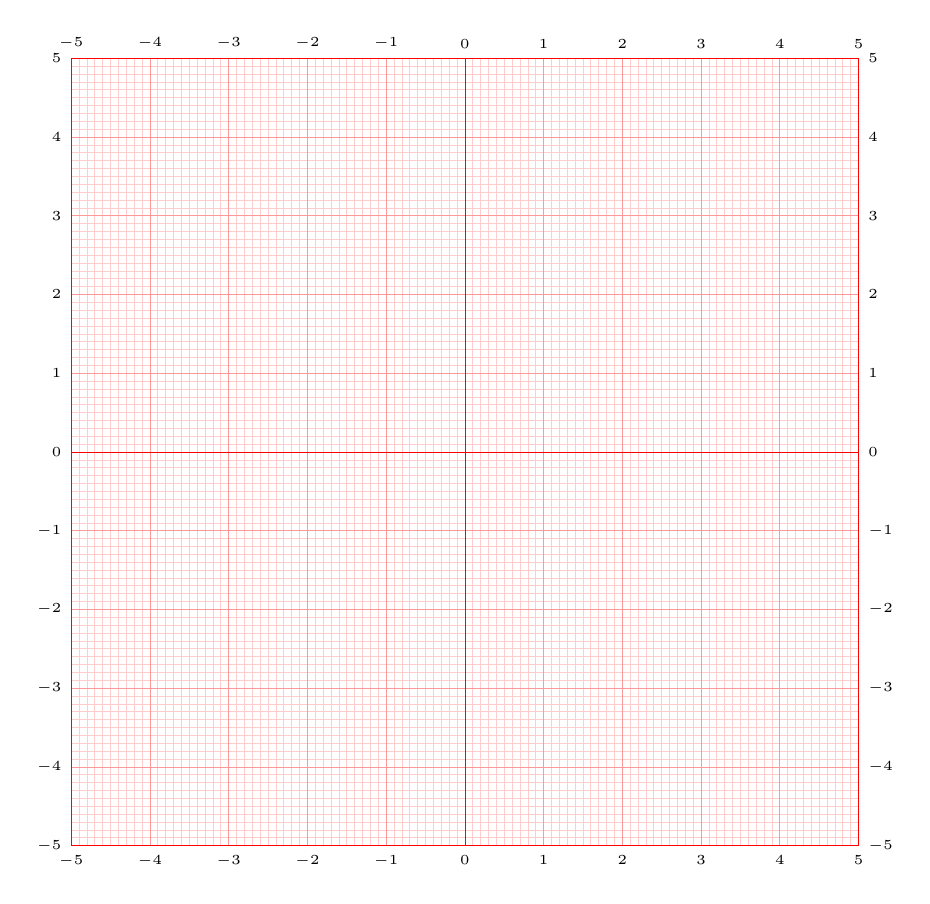
\begin{tikzpicture}
  % a grid with default values
  \mygrid
\end{tikzpicture}
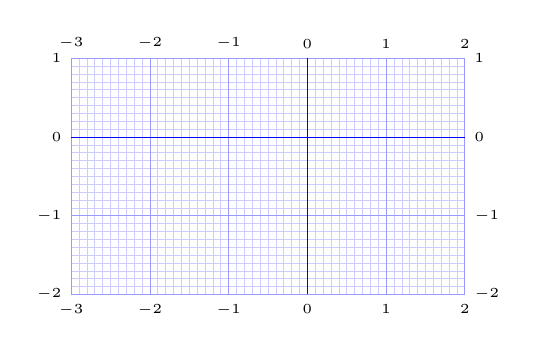
\begin{tikzpicture}
  % a grid with specific values 
  \mygrid[min x=-3, max x=2,min y=-2,max y=1,color=blue]
\end{tikzpicture}
\begin{tikzpicture}
  % a grid using the `a grid` style
  \mygrid[a grid]
\end{tikzpicture}
\end{document}
